\documentclass[10pt]{article}
\usepackage{arxiv}
\usepackage[T1]{fontenc}
\usepackage{microtype,amsmath,amssymb,graphicx,booktabs,array,tabularx}
\usepackage[numbers,sort&compress]{natbib}
\usepackage[hidelinks]{hyperref}
\usepackage{float}
\floatstyle{ruled}\newfloat{algorithm}{t}{loa}\floatname{algorithm}{Algorithm}
\hypersetup{pdftitle={Which Better Schedule Can the Vehicles Adopt? Safe Revision, Recovery and Commitment at Autonomous Intersections},
  pdfauthor={Nishchay Bhutoria, Tanish Wanve, Swayam Borate, D A S K R Manognya}}

% Header and title block in the layout of the project-review report.
\renewcommand{\headeright}{CS 329: Foundations of AI: Multiagent Systems}
\renewcommand{\shorttitle}{}
\fancyhead[R]{\small\itshape\headeright}
\renewcommand{\undertitle}{Final Project Report}
\makeatletter
\renewcommand{\@seccntformat}[1]{\csname the#1\endcsname.\quad}
\renewcommand{\@maketitle}{%
  \vbox{\hsize\textwidth\linewidth\hsize\centering
    {\LARGE\bfseries \@title\par}\vskip 0.08in
    {\large \undertitle\par}\vskip 0.06in
    {\normalsize \@author\par}\vskip 0.06in
    {\normalsize \@date\par}\vskip 0.12in}}
\makeatother

\title{Which Better Schedule Can the Vehicles Adopt?\\Safe Revision, Recovery and Commitment at Autonomous Intersections}
\author{\begin{tabular}{@{}l@{\hspace{1.2em}}l@{}}
\textbf{Nishchay Bhutoria} & 23110222\\ \textbf{Tanish Wanve} & 23110327\\
\textbf{Swayam Borate} & 23110066\\ \textbf{D A S K R Manognya} & 24110097\end{tabular}}
\date{\textbf{CS 329: Foundations of AI: Multiagent Systems}\\Indian Institute of Technology Gandhinagar}

% Generated by experiments/reproduce_report.py from results/data; do not edit by hand.
\newcommand{\nCommitCells}{24}
\newcommand{\nCommitNeverFreeze}{24}
\newcommand{\nCommitTestRuns}{1{,}800}
\newcommand{\nCommitTuneRuns}{3{,}072}
\newcommand{\nFcfsMax}{0.44}
\newcommand{\nFcfsMin}{0.16}
\newcommand{\nFcfsMinusRolling}{0.31}
\newcommand{\nFcfsMinusRollingAbs}{0.31}
\newcommand{\nFcfsMinusRollingHi}{0.39}
\newcommand{\nFcfsMinusRollingLo}{0.23}
\newcommand{\nFreezeFourMax}{0.11}
\newcommand{\nFreezeFourMaxThree}{0.108}
\newcommand{\nFreezeFourMin}{0.04}
\newcommand{\nFreezeFourMinThree}{0.035}
\newcommand{\nFreezeFourMinusRolling}{0.073}
\newcommand{\nFreezeFourMinusRollingAbs}{0.073}
\newcommand{\nFreezeFourMinusRollingHi}{0.093}
\newcommand{\nFreezeFourMinusRollingLo}{0.056}
\newcommand{\nFreezeInfMax}{0.56}
\newcommand{\nFreezeInfMin}{0.16}
\newcommand{\nFreezeInfMinusRolling}{0.38}
\newcommand{\nFreezeInfMinusRollingAbs}{0.38}
\newcommand{\nFreezeInfMinusRollingHi}{0.44}
\newcommand{\nFreezeInfMinusRollingLo}{0.33}
\newcommand{\nPairCross}{12.4}
\newcommand{\nPairNine}{1.18}
\newcommand{\nRtAwareMax}{0.015}
\newcommand{\nRtAwareMinHolm}{0.59}
\newcommand{\nRtBurstOne}{\ensuremath{-}0.49}
\newcommand{\nRtBurstOneAbs}{0.49}
\newcommand{\nRtBurstOneHi}{\ensuremath{-}0.41}
\newcommand{\nRtBurstOneLo}{\ensuremath{-}0.57}
\newcommand{\nRtBurstTwo}{\ensuremath{-}0.89}
\newcommand{\nRtBurstTwoAbs}{0.89}
\newcommand{\nRtBurstTwoHi}{\ensuremath{-}0.79}
\newcommand{\nRtBurstTwoLo}{\ensuremath{-}0.99}
\newcommand{\nRtDetourTwoHigh}{\ensuremath{-}0.15}
\newcommand{\nRtDetourTwoHighAbs}{0.15}
\newcommand{\nRtDetourTwoHighHi}{\ensuremath{-}0.10}
\newcommand{\nRtDetourTwoHighLo}{\ensuremath{-}0.19}
\newcommand{\nRtDetourTwoLow}{\ensuremath{-}0.10}
\newcommand{\nRtDetourTwoLowAbs}{0.10}
\newcommand{\nRtDetourTwoLowHi}{\ensuremath{-}0.07}
\newcommand{\nRtDetourTwoLowLo}{\ensuremath{-}0.13}
\newcommand{\nRtDetourTwoPriceHigh}{0.22}
\newcommand{\nRtDetourTwoPriceHighAbs}{0.22}
\newcommand{\nRtDetourTwoPriceHighHi}{0.28}
\newcommand{\nRtDetourTwoPriceHighLo}{0.16}
\newcommand{\nRtDetourTwoPriceLow}{0.13}
\newcommand{\nRtDetourTwoPriceLowAbs}{0.13}
\newcommand{\nRtDetourTwoPriceLowHi}{0.16}
\newcommand{\nRtDetourTwoPriceLowLo}{0.11}
\newcommand{\nRtDetourZeroHigh}{+0.09}
\newcommand{\nRtDetourZeroHighAbs}{0.09}
\newcommand{\nRtDetourZeroHighHi}{+0.16}
\newcommand{\nRtDetourZeroHighLo}{+0.03}
\newcommand{\nRtDetourZeroLow}{+0.08}
\newcommand{\nRtDetourZeroLowAbs}{0.08}
\newcommand{\nRtDetourZeroLowHi}{+0.12}
\newcommand{\nRtDetourZeroLowLo}{+0.04}
\newcommand{\nRtExtraRoundsOne}{47}
\newcommand{\nRtExtraRoundsTwo}{61}
\newcommand{\nRtFreezeOneHigh}{+0.09}
\newcommand{\nRtFreezeOneHighAbs}{0.09}
\newcommand{\nRtFreezeOneHighHi}{+0.14}
\newcommand{\nRtFreezeOneHighLo}{+0.04}
\newcommand{\nRtFreezeOneLow}{+0.08}
\newcommand{\nRtFreezeOneLowAbs}{0.08}
\newcommand{\nRtFreezeOneLowHi}{+0.12}
\newcommand{\nRtFreezeOneLowLo}{+0.05}
\newcommand{\nRtFreezeZeroHigh}{+0.06}
\newcommand{\nRtFreezeZeroHighAbs}{0.06}
\newcommand{\nRtFreezeZeroHighHi}{+0.10}
\newcommand{\nRtFreezeZeroHighLo}{+0.03}
\newcommand{\nRtFreezeZeroLow}{+0.07}
\newcommand{\nRtFreezeZeroLowAbs}{0.07}
\newcommand{\nRtFreezeZeroLowHi}{+0.10}
\newcommand{\nRtFreezeZeroLowLo}{+0.03}
\newcommand{\nRtGrantsOne}{265}
\newcommand{\nRtGrantsOracle}{296}
\newcommand{\nRtGrantsTwo}{273}
\newcommand{\nRtGrantsZero}{202}
\newcommand{\nRtMeanAtomic}{4.92}
\newcommand{\nRtModelOne}{19}
\newcommand{\nRtModelRecOne}{81}
\newcommand{\nRtModelRecTwo}{96.4}
\newcommand{\nRtModelTwo}{3.6}
\newcommand{\nRtOneRetryTenHigh}{\ensuremath{-}1.13}
\newcommand{\nRtOneRetryTenHighAbs}{1.13}
\newcommand{\nRtOneRetryTenHighHi}{\ensuremath{-}1.02}
\newcommand{\nRtOneRetryTenHighLo}{\ensuremath{-}1.24}
\newcommand{\nRtOneRetryTenLow}{\ensuremath{-}0.87}
\newcommand{\nRtOneRetryTenLowAbs}{0.87}
\newcommand{\nRtOneRetryTenLowHi}{\ensuremath{-}0.81}
\newcommand{\nRtOneRetryTenLowLo}{\ensuremath{-}0.94}
\newcommand{\nRtPFiveAtomic}{17.2}
\newcommand{\nRtPFiveOne}{15.7}
\newcommand{\nRtPFiveOracle}{15.4}
\newcommand{\nRtPFiveTwo}{15.5}
\newcommand{\nRtPFiveZero}{17.2}
\newcommand{\nRtPinShareOne}{3.5}
\newcommand{\nRtPinShareOracle}{0.0}
\newcommand{\nRtPinShareTwo}{0.6}
\newcommand{\nRtPinShareZero}{19.1}
\newcommand{\nRtPinnedOne}{9.2}
\newcommand{\nRtPinnedOracle}{0.0}
\newcommand{\nRtPinnedTwo}{1.6}
\newcommand{\nRtPinnedZero}{38.6}
\newcommand{\nRtPriceOneCleanHigh}{0.34}
\newcommand{\nRtPriceOneCleanHighAbs}{0.34}
\newcommand{\nRtPriceOneCleanHighHi}{0.40}
\newcommand{\nRtPriceOneCleanHighLo}{0.28}
\newcommand{\nRtPriceOneCleanLow}{0.22}
\newcommand{\nRtPriceOneCleanLowAbs}{0.22}
\newcommand{\nRtPriceOneCleanLowHi}{0.25}
\newcommand{\nRtPriceOneCleanLowLo}{0.19}
\newcommand{\nRtPriceOneTenHigh}{0.53}
\newcommand{\nRtPriceOneTenHighAbs}{0.53}
\newcommand{\nRtPriceOneTenHighHi}{0.59}
\newcommand{\nRtPriceOneTenHighLo}{0.46}
\newcommand{\nRtPriceOneTenLow}{0.39}
\newcommand{\nRtPriceOneTenLowAbs}{0.39}
\newcommand{\nRtPriceOneTenLowHi}{0.44}
\newcommand{\nRtPriceOneTenLowLo}{0.35}
\newcommand{\nRtPriceOneTwentyHigh}{1.11}
\newcommand{\nRtPriceOneTwentyHighAbs}{1.11}
\newcommand{\nRtPriceOneTwentyHighHi}{1.21}
\newcommand{\nRtPriceOneTwentyHighLo}{1.01}
\newcommand{\nRtPriceOneTwentyLow}{0.84}
\newcommand{\nRtPriceOneTwentyLowAbs}{0.84}
\newcommand{\nRtPriceOneTwentyLowHi}{0.91}
\newcommand{\nRtPriceOneTwentyLowLo}{0.78}
\newcommand{\nRtPriceOracleCleanHigh}{0.34}
\newcommand{\nRtPriceOracleCleanHighAbs}{0.34}
\newcommand{\nRtPriceOracleCleanHighHi}{0.40}
\newcommand{\nRtPriceOracleCleanHighLo}{0.28}
\newcommand{\nRtPriceOracleCleanLow}{0.22}
\newcommand{\nRtPriceOracleCleanLowAbs}{0.22}
\newcommand{\nRtPriceOracleCleanLowHi}{0.25}
\newcommand{\nRtPriceOracleCleanLowLo}{0.19}
\newcommand{\nRtPriceOracleTenHigh}{0.34}
\newcommand{\nRtPriceOracleTenHighAbs}{0.34}
\newcommand{\nRtPriceOracleTenHighHi}{0.40}
\newcommand{\nRtPriceOracleTenHighLo}{0.28}
\newcommand{\nRtPriceOracleTenLow}{0.23}
\newcommand{\nRtPriceOracleTenLowAbs}{0.23}
\newcommand{\nRtPriceOracleTenLowHi}{0.26}
\newcommand{\nRtPriceOracleTenLowLo}{0.20}
\newcommand{\nRtPriceOracleTwentyHigh}{0.37}
\newcommand{\nRtPriceOracleTwentyHighAbs}{0.37}
\newcommand{\nRtPriceOracleTwentyHighHi}{0.43}
\newcommand{\nRtPriceOracleTwentyHighLo}{0.31}
\newcommand{\nRtPriceOracleTwentyLow}{0.26}
\newcommand{\nRtPriceOracleTwentyLowAbs}{0.26}
\newcommand{\nRtPriceOracleTwentyLowHi}{0.30}
\newcommand{\nRtPriceOracleTwentyLowLo}{0.23}
\newcommand{\nRtPriceTwoCleanHigh}{0.34}
\newcommand{\nRtPriceTwoCleanHighAbs}{0.34}
\newcommand{\nRtPriceTwoCleanHighHi}{0.40}
\newcommand{\nRtPriceTwoCleanHighLo}{0.28}
\newcommand{\nRtPriceTwoCleanLow}{0.22}
\newcommand{\nRtPriceTwoCleanLowAbs}{0.22}
\newcommand{\nRtPriceTwoCleanLowHi}{0.25}
\newcommand{\nRtPriceTwoCleanLowLo}{0.19}
\newcommand{\nRtPriceTwoTenHigh}{0.36}
\newcommand{\nRtPriceTwoTenHighAbs}{0.36}
\newcommand{\nRtPriceTwoTenHighHi}{0.43}
\newcommand{\nRtPriceTwoTenHighLo}{0.30}
\newcommand{\nRtPriceTwoTenLow}{0.23}
\newcommand{\nRtPriceTwoTenLowAbs}{0.23}
\newcommand{\nRtPriceTwoTenLowHi}{0.27}
\newcommand{\nRtPriceTwoTenLowLo}{0.20}
\newcommand{\nRtPriceTwoTwentyHigh}{0.58}
\newcommand{\nRtPriceTwoTwentyHighAbs}{0.58}
\newcommand{\nRtPriceTwoTwentyHighHi}{0.67}
\newcommand{\nRtPriceTwoTwentyHighLo}{0.51}
\newcommand{\nRtPriceTwoTwentyLow}{0.42}
\newcommand{\nRtPriceTwoTwentyLowAbs}{0.42}
\newcommand{\nRtPriceTwoTwentyLowHi}{0.46}
\newcommand{\nRtPriceTwoTwentyLowLo}{0.38}
\newcommand{\nRtPriceZeroCleanHigh}{0.34}
\newcommand{\nRtPriceZeroCleanHighAbs}{0.34}
\newcommand{\nRtPriceZeroCleanHighHi}{0.40}
\newcommand{\nRtPriceZeroCleanHighLo}{0.28}
\newcommand{\nRtPriceZeroCleanLow}{0.22}
\newcommand{\nRtPriceZeroCleanLowAbs}{0.22}
\newcommand{\nRtPriceZeroCleanLowHi}{0.25}
\newcommand{\nRtPriceZeroCleanLowLo}{0.19}
\newcommand{\nRtPriceZeroTenHigh}{1.66}
\newcommand{\nRtPriceZeroTenHighAbs}{1.66}
\newcommand{\nRtPriceZeroTenHighHi}{1.77}
\newcommand{\nRtPriceZeroTenHighLo}{1.54}
\newcommand{\nRtPriceZeroTenLow}{1.27}
\newcommand{\nRtPriceZeroTenLowAbs}{1.27}
\newcommand{\nRtPriceZeroTenLowHi}{1.35}
\newcommand{\nRtPriceZeroTenLowLo}{1.19}
\newcommand{\nRtPriceZeroTwentyHigh}{2.37}
\newcommand{\nRtPriceZeroTwentyHighAbs}{2.37}
\newcommand{\nRtPriceZeroTwentyHighHi}{2.50}
\newcommand{\nRtPriceZeroTwentyHighLo}{2.24}
\newcommand{\nRtPriceZeroTwentyLow}{1.93}
\newcommand{\nRtPriceZeroTwentyLowAbs}{1.93}
\newcommand{\nRtPriceZeroTwentyLowHi}{2.02}
\newcommand{\nRtPriceZeroTwentyLowLo}{1.85}
\newcommand{\nRtPrimary}{\ensuremath{-}1.13}
\newcommand{\nRtPrimaryAbs}{1.13}
\newcommand{\nRtPrimaryHi}{\ensuremath{-}1.02}
\newcommand{\nRtPrimaryLo}{\ensuremath{-}1.24}
\newcommand{\nRtPrimaryP}{10^{-4}}
\newcommand{\nRtRecAmpleOne}{82}
\newcommand{\nRtRecAmpleTwo}{97}
\newcommand{\nRtRecOne}{68}
\newcommand{\nRtRecOneAbs}{68}
\newcommand{\nRtRecOneHi}{72}
\newcommand{\nRtRecOneLo}{64}
\newcommand{\nRtRecOracle}{80}
\newcommand{\nRtRecOracleAbs}{80}
\newcommand{\nRtRecOracleHi}{83}
\newcommand{\nRtRecOracleLo}{76}
\newcommand{\nRtRecTwo}{78}
\newcommand{\nRtRecTwoAbs}{78}
\newcommand{\nRtRecTwoHi}{82}
\newcommand{\nRtRecTwoLo}{74}
\newcommand{\nRtRetxOne}{50}
\newcommand{\nRtRetxShareOne}{19}
\newcommand{\nRtRetxShareTwo}{23}
\newcommand{\nRtRetxTwo}{62}
\newcommand{\nRtRuns}{8{,}520}
\newcommand{\nRtSecondTenHigh}{\ensuremath{-}0.16}
\newcommand{\nRtSecondTenHighAbs}{0.16}
\newcommand{\nRtSecondTenHighHi}{\ensuremath{-}0.13}
\newcommand{\nRtSecondTenHighLo}{\ensuremath{-}0.20}
\newcommand{\nRtSecondTenLow}{\ensuremath{-}0.16}
\newcommand{\nRtSecondTenLowAbs}{0.16}
\newcommand{\nRtSecondTenLowHi}{\ensuremath{-}0.13}
\newcommand{\nRtSecondTenLowLo}{\ensuremath{-}0.19}
\newcommand{\nRtSecondTwentyHigh}{\ensuremath{-}0.53}
\newcommand{\nRtSecondTwentyHighAbs}{0.53}
\newcommand{\nRtSecondTwentyHighHi}{\ensuremath{-}0.45}
\newcommand{\nRtSecondTwentyHighLo}{\ensuremath{-}0.61}
\newcommand{\nRtSecondTwentyLow}{\ensuremath{-}0.42}
\newcommand{\nRtSecondTwentyLowAbs}{0.42}
\newcommand{\nRtSecondTwentyLowHi}{\ensuremath{-}0.38}
\newcommand{\nRtSecondTwentyLowLo}{\ensuremath{-}0.47}
\newcommand{\nRtSlotFiftyOneHigh}{\ensuremath{-}1.13}
\newcommand{\nRtSlotFiftyOneHighAbs}{1.13}
\newcommand{\nRtSlotFiftyOneHighHi}{\ensuremath{-}1.02}
\newcommand{\nRtSlotFiftyOneHighLo}{\ensuremath{-}1.25}
\newcommand{\nRtSlotFiftyOneLow}{\ensuremath{-}0.88}
\newcommand{\nRtSlotFiftyOneLowAbs}{0.88}
\newcommand{\nRtSlotFiftyOneLowHi}{\ensuremath{-}0.81}
\newcommand{\nRtSlotFiftyOneLowLo}{\ensuremath{-}0.94}
\newcommand{\nRtSlotHalfOneHigh}{\ensuremath{-}0.91}
\newcommand{\nRtSlotHalfOneHighAbs}{0.91}
\newcommand{\nRtSlotHalfOneHighHi}{\ensuremath{-}0.82}
\newcommand{\nRtSlotHalfOneHighLo}{\ensuremath{-}1.00}
\newcommand{\nRtSlotHalfOneLow}{\ensuremath{-}0.74}
\newcommand{\nRtSlotHalfOneLowAbs}{0.74}
\newcommand{\nRtSlotHalfOneLowHi}{\ensuremath{-}0.68}
\newcommand{\nRtSlotHalfOneLowLo}{\ensuremath{-}0.80}
\newcommand{\nRtSlotSecondOneHigh}{\ensuremath{-}0.59}
\newcommand{\nRtSlotSecondOneHighAbs}{0.59}
\newcommand{\nRtSlotSecondOneHighHi}{\ensuremath{-}0.51}
\newcommand{\nRtSlotSecondOneHighLo}{\ensuremath{-}0.67}
\newcommand{\nRtSlotSecondOneLow}{\ensuremath{-}0.41}
\newcommand{\nRtSlotSecondOneLowAbs}{0.41}
\newcommand{\nRtSlotSecondOneLowHi}{\ensuremath{-}0.36}
\newcommand{\nRtSlotSecondOneLowLo}{\ensuremath{-}0.46}
\newcommand{\nRtSlotSecondPriceOracleHigh}{1.39}
\newcommand{\nRtSlotSecondPriceOracleHighAbs}{1.39}
\newcommand{\nRtSlotSecondPriceOracleHighHi}{1.51}
\newcommand{\nRtSlotSecondPriceOracleHighLo}{1.28}
\newcommand{\nRtSlotSecondPriceOracleLow}{1.12}
\newcommand{\nRtSlotSecondPriceOracleLowAbs}{1.12}
\newcommand{\nRtSlotSecondPriceOracleLowHi}{1.20}
\newcommand{\nRtSlotSecondPriceOracleLowLo}{1.04}
\newcommand{\nRtSlotSecondPriceTwoHigh}{1.30}
\newcommand{\nRtSlotSecondPriceTwoHighAbs}{1.30}
\newcommand{\nRtSlotSecondPriceTwoHighHi}{1.42}
\newcommand{\nRtSlotSecondPriceTwoHighLo}{1.19}
\newcommand{\nRtSlotSecondPriceTwoLow}{1.12}
\newcommand{\nRtSlotSecondPriceTwoLowAbs}{1.12}
\newcommand{\nRtSlotSecondPriceTwoLowHi}{1.18}
\newcommand{\nRtSlotSecondPriceTwoLowLo}{1.05}
\newcommand{\nRtSlotSecondPriceZeroHigh}{1.94}
\newcommand{\nRtSlotSecondPriceZeroHighAbs}{1.94}
\newcommand{\nRtSlotSecondPriceZeroHighHi}{2.07}
\newcommand{\nRtSlotSecondPriceZeroHighLo}{1.80}
\newcommand{\nRtSlotSecondPriceZeroLow}{1.56}
\newcommand{\nRtSlotSecondPriceZeroLowAbs}{1.56}
\newcommand{\nRtSlotSecondPriceZeroLowHi}{1.65}
\newcommand{\nRtSlotSecondPriceZeroLowLo}{1.48}
\newcommand{\nRtSlotSecondTwoOracleHigh}{\ensuremath{-}0.09}
\newcommand{\nRtSlotSecondTwoOracleHighAbs}{0.09}
\newcommand{\nRtSlotSecondTwoOracleHighHi}{\ensuremath{-}0.02}
\newcommand{\nRtSlotSecondTwoOracleHighLo}{\ensuremath{-}0.16}
\newcommand{\nRtSlotSecondTwoOracleHolmHigh}{0.28}
\newcommand{\nRtSpareThreeFifty}{100}
\newcommand{\nRtSpareThreeHalf}{84}
\newcommand{\nRtSpareThreeQuarter}{96}
\newcommand{\nRtSpareThreeSecond}{44}
\newcommand{\nRtSpareThreeTenth}{99}
\newcommand{\nRtSpareZeroFifty}{0}
\newcommand{\nRtSpareZeroHalf}{4}
\newcommand{\nRtSpareZeroQuarter}{1}
\newcommand{\nRtSpareZeroSecond}{16}
\newcommand{\nRtSpareZeroTenth}{0}
\newcommand{\nRtStreams}{60}
\newcommand{\nRtTwoTenMinusCleanHigh}{+0.03}
\newcommand{\nRtTwoTenMinusCleanHighAbs}{0.03}
\newcommand{\nRtTwoTenMinusCleanHighHi}{+0.06}
\newcommand{\nRtTwoTenMinusCleanHighLo}{+0.01}
\newcommand{\nRtTwoTenMinusCleanLow}{+0.02}
\newcommand{\nRtTwoTenMinusCleanLowAbs}{0.02}
\newcommand{\nRtTwoTenMinusCleanLowHi}{+0.02}
\newcommand{\nRtTwoTenMinusCleanLowLo}{+0.01}
\newcommand{\nRtTwoTwentyMinusCleanHigh}{+0.25}
\newcommand{\nRtTwoTwentyMinusCleanHighAbs}{0.25}
\newcommand{\nRtTwoTwentyMinusCleanHighHi}{+0.32}
\newcommand{\nRtTwoTwentyMinusCleanHighLo}{+0.18}
\newcommand{\nRtTwoTwentyMinusCleanLow}{+0.20}
\newcommand{\nRtTwoTwentyMinusCleanLowAbs}{0.20}
\newcommand{\nRtTwoTwentyMinusCleanLowHi}{+0.23}
\newcommand{\nRtTwoTwentyMinusCleanLowLo}{+0.17}
\newcommand{\nRtVsFcfsTwoTenHigh}{\ensuremath{-}0.06}
\newcommand{\nRtVsFcfsTwoTenHighAbs}{0.06}
\newcommand{\nRtVsFcfsTwoTenHighHi}{\ensuremath{-}0.01}
\newcommand{\nRtVsFcfsTwoTenHighLo}{\ensuremath{-}0.12}
\newcommand{\nRtVsFcfsTwoTenHolmHigh}{0.084}
\newcommand{\nRtVsFcfsTwoTenHolmLow}{0.007}
\newcommand{\nRtVsFcfsTwoTenLow}{\ensuremath{-}0.05}
\newcommand{\nRtVsFcfsTwoTenLowAbs}{0.05}
\newcommand{\nRtVsFcfsTwoTenLowHi}{\ensuremath{-}0.02}
\newcommand{\nRtVsFcfsTwoTenLowLo}{\ensuremath{-}0.09}
\newcommand{\nRtZeroSpareQueried}{59}
\newcommand{\nStopMax}{0.0004}
\newcommand{\nStopMin}{0.0000}
\newcommand{\nStopMinusTuned}{8.1}
\newcommand{\nStopMinusTunedAbs}{8.1}
\newcommand{\nStopMinusTunedHi}{20.5}
\newcommand{\nStopMinusTunedLo}{0.7}
\newcommand{\nStopSignificant}{0}
\newcommand{\nSweepAwareNonNeg}{12}
\newcommand{\nSweepForks}{23{,}472}
\newcommand{\nSweepGainMax}{497}
\newcommand{\nSweepGainMin}{64}
\newcommand{\nSweepGapNineMax}{89.9}
\newcommand{\nSweepGapNineMin}{15.5}
\newcommand{\nSweepGapNineShareMax}{28}
\newcommand{\nSweepGapPerfectMax}{31.9}
\newcommand{\nSweepGapPerfectMin}{4.6}
\newcommand{\nSweepGapPerfectShareMax}{15}
\newcommand{\nSweepImproving}{5{,}473}
\newcommand{\nSweepMenuMax}{0.80}
\newcommand{\nSweepMinHolm}{0.46}
\newcommand{\nSweepObliviousMax}{\ensuremath{-}0.9}
\newcommand{\nSweepObliviousMin}{\ensuremath{-}20.5}
\newcommand{\nSweepObliviousNeg}{7}
\newcommand{\nSweepObliviousNegEst}{12}
\newcommand{\nSweepPrimary}{+5.6}
\newcommand{\nSweepPrimaryAbs}{5.6}
\newcommand{\nSweepPrimaryForks}{2{,}057}
\newcommand{\nSweepPrimaryHi}{+13.0}
\newcommand{\nSweepPrimaryLo}{\ensuremath{-}0.5}
\newcommand{\nSweepRecMax}{29.9}
\newcommand{\nSweepRecMin}{4.6}
\newcommand{\nSweepReorderShare}{12}
\newcommand{\nSweepReorders}{678}
\newcommand{\nSweepRescued}{609}
\newcommand{\nSweepRescuedShare}{90}
\newcommand{\nSweepShortDirect}{678}
\newcommand{\nSweepStillShort}{69}
\newcommand{\nSweepStreams}{384}
\newcommand{\nTuneCurveMin}{0.000}
\newcommand{\nTuneCurveNeg}{0}

\newcommand{\E}{\mathbb{E}}

\begin{document}\raggedbottom
\maketitle

\begin{abstract}
Connected and automated vehicles can cross a signal-free intersection on reserved time slots that a coordinator keeps re-optimizing as information improves. A better schedule helps only if the vehicles can adopt it: each change must be installed message by message, without ever authorizing two conflicting reservations, over a link that loses messages, and while each vehicle can still physically make the change. We formulate this multiagent coordination problem and study it in a two-lane reservation simulator with exact rolling optimization, a release-gated update protocol, temporary reservations and bounded, version-safe retransmission. Locking crossing orders early never helped: tuning chose \emph{never lock} in all \nCommitCells{} traffic and noise regimes. On a perfect link, safe installation fell short of an idealized atomic update exactly at the \nSweepReorders{} decisions that reversed a tightly spaced pair, which creates a cycle of release dependencies; one temporary reservation repaired \nSweepRescued{} of them. In sustained traffic with 10\% loss per message, one-attempt safe installation cost \nRtPriceZeroTenHigh{} s per vehicle against the idealized update. One retry recovered \nRtPrimaryAbs{} s of this (\nRtRecOne\%), two retries came within \nRtTwoTenMinusCleanHighAbs{} s of a loss-free link, and physical deadlines limited recovery only for message slots of 0.5 s or longer.
\end{abstract}

\section{Introduction}
Connected and automated vehicles (CAVs) can share an intersection without traffic lights: an intersection manager assigns each vehicle a reserved entry time so that vehicles from conflicting approaches never occupy the crossing together~\cite{dresner2008}. Because crossing times are planned jointly, the manager solves a sequencing problem over all approaching vehicles, and it can re-solve it whenever predicted arrival times improve~\cite{liwang2006,miculescu2020,chalaki2022,vitale2023}. Re-optimization, however, only produces a \emph{nominal} schedule. Whether vehicles can move to it depends on the reservations they already hold.

Vehicle A is booked to enter at 10 s, and vehicle B on the other approach at 14 s; conflicting entries need 3 s of clearance. New information shows that B could enter at 9 s. Sending B at 9 and A at 12 saves three vehicle-seconds, yet no instruction can be sent first: granting B 9 s while A holds 10 s violates clearance, and so does granting A 12 s while B holds 14 s (Fig.~\ref{fig:handoff}a). A reservation is a commitment that is discharged only when its vehicle confirms that it has moved, so each new booking waits for the release of another, and reversing a tightly spaced pair creates a \emph{cycle} of such dependencies. A temporary reservation breaks the cycle (park B at 15 s, move A to 12 s, return B to 9 s; Fig.~\ref{fig:handoff}b) at the cost of three dependent messages instead of two.

Messages can also be lost. If the manager hears nothing after granting A 12 s, it cannot tell whether the grant was lost (A still holds 10 s) or the acknowledgment was (A holds 12 s). It must keep both reservations clear, so A becomes \emph{ambiguous} and blocks others. Asking again resolves the ambiguity, but each attempt costs a round trip, and a switch can be commanded only while the vehicle can still physically execute it; simultaneous switching cannot be guaranteed over a lossy link at all~\cite{twogenerals}.

We therefore ask: \emph{how can autonomous vehicles safely adopt improved cooperative crossing schedules when existing reservations, communication uncertainty and physical feasibility constrain plan changes?} Prior intersection work decides \emph{when} to resequence~\cite{chalaki2022,vitale2023,berndt2024}, assumes reliable or delay-bounded messaging~\cite{zheng19,au2011}, or fixes actuation times to tolerate delay~\cite{crossroads}. Network updates and parallel register moves handle release dependencies with dependency graphs and temporaries~\cite{reitblatt2012,jin2014,rideau2008}, and solution stability is a known concern in dynamic constraint optimization~\cite{petcu2007}. Our objectives and contributions are:
(i) a formulation of safe schedule revision in which a coordinator and vehicle agents exchange grants and acknowledgments under clearance, ordering, motion and communication constraints;
(ii) algorithms for rolling exact scheduling with fixed and adaptive order commitment, release-gated installation scored by its exact expected value, temporary reservations, and version-safe bounded retransmission; and
(iii) a reproducible evaluation in three simulation studies that separates the costs of commitment, release cycles, message loss and physical deadlines.

\begin{figure}[t]\centering
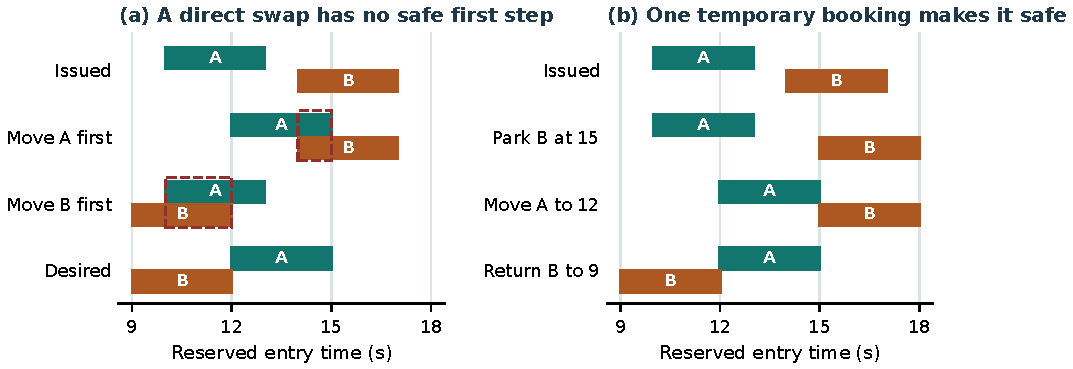
\includegraphics[width=.86\linewidth]{figures/fig1_handoff.pdf}
\caption{\textbf{The two-vehicle example.} Boxes are 3 s occupancy intervals. (a) Moving either vehicle first overlaps the other's still-valid reservation (dashed). (b) With a temporary reservation, each step differs from the previous one by a single executable, acknowledged booking.}\label{fig:handoff}
\end{figure}

\section{Preliminaries}\label{sec:prelim}
\paragraph{Vehicles and information.} Two single-lane approaches share one conflict zone, and vehicles cannot overtake (FIFO per lane). Vehicle $i$ requests a reservation at time $a_i$; requests form a Poisson stream split equally between lanes with offered load $\rho=\lambda h$ ($\lambda$: total arrival rate). Vehicle $i$ can enter no earlier than its private readiness time $r_i=a_i+L_0+\sigma\sum_{k=1}^{4}Z_{ik}$, where the signs $Z_{ik}\in\{-1,+1\}$ are revealed publicly one per second. After $k$ revelations the public guard
\begin{equation}
U_i(k)=a_i+L_0+\sigma\Big(\textstyle\sum_{m\le k}Z_{im}+4-k\Big)\ \ge\ r_i \label{eq:guard}
\end{equation}
never increases, so a reservation at or after $U_i$ stays valid whatever is revealed later, and each negative sign lets the schedule improve by $2\sigma$.

\paragraph{Motion, headways and schedules.} Vehicles have bounded acceleration $\alpha$, braking $b$ and speed $V$ on an approach of length $L$; the head of each lane has a window $W_i(t)$ of reachable entry times, and followers launch from rest when their predecessor enters, needing at least $T_L$. A reservation is an entry time $s_i$. Entries from different lanes must be at least $h$ apart and same-lane entries at least $\max(h_f,T_L)$; two reservations are \emph{compatible} if they respect these headways. A schedule $s$ is \emph{feasible} at time $t$ if $s_i\ge U_i(t)$, $s_i\in W_i(t)$, lanes stay FIFO and all pairs are compatible. Commitments are precedence locks $(i\prec j)\in C_t$ with $C_t\subseteq C_{t+1}$.

\paragraph{Messages and reservations.} The manager changes vehicle $i$'s booking from $O_i$ to $T_i$ by a \emph{grant}; the vehicle switches at a fixed instant and replies with an acknowledgment (ACK). Grants are delivered with probability $u$ and replies with probability $v$, independently, in one-way slots of length $d$; we write $u=v=1-q$ for a loss rate $q$ per leg. For each vehicle the manager keeps a \emph{protected set} $P_i$ of bookings that others must avoid: $\{O_i\}$ normally and $\{O_i,T_i\}$ while a grant is unconfirmed. Removing a booking from $P_i$ is a \emph{release}. Vehicle $i$'s delay is $S_i-r_i$, where $S_i$ is its actual entry time.

\section{Problem Formulation}\label{sec:problem}
\paragraph{Agents, states and information.} An intersection manager $M$ coordinates cooperative vehicle agents $i\in\mathcal V_t$. The state comprises the vehicles' physical states, issued bookings $O$, protected sets $P$, locks $C_t$, the public information $(a_i,U_i(t))$ and messages in flight. $M$ observes requests, public signals, the replies it receives and entries, but never $r_i$ or which message was lost. A vehicle knows its own state and the grants it has received, and executes every valid grant.

\paragraph{Decisions.} At each event (request, signal, entry, end of an installation round) $M$ chooses (i) a nominal target schedule, (ii) whether to add locks to $C_t$, (iii) an installation plan, i.e.\ a set of single-vehicle booking changes (\emph{moves}), possibly via one temporary booking, each issued once the moves it depends on are acknowledged, and (iv) for each unconfirmed move, whether to retransmit it or query the vehicle, within $K$ extra transmissions. The rolling target is
\begin{equation}
N(t)\in\arg\min_{s}\ \textstyle\sum_{i\in\mathcal V_t}s_i \quad\text{s.t. } s \text{ feasible at } t,\ \ (i\prec j)\in C_t\Rightarrow s_j\ge s_i+h, \label{eq:target}
\end{equation}
with the protected bookings of unrevisable vehicles as fixed blocks. Since $r_i$ is fixed, this minimizes the total delay of the scheduled vehicles.

\paragraph{Safety constraints (hard).} All protected bookings of different vehicles are pairwise compatible at all times; a grant $O_i\to T_i$ is sent only if $T_i$ is compatible with every booking still protected for others; a switch is commanded only if the vehicle can physically execute it at its switch instant; and a booking is released only on an ACK, a void report or an observed entry, never on silence or elapsed time. Safety therefore never depends on message delivery.

\paragraph{Objective, uncertainty and resources.} $M$ minimizes the expected mean delay of a cohort $\mathcal I$ in sustained traffic, $\E\big[|\mathcal I|^{-1}\sum_{i\in\mathcal I}(S_i-r_i)\big]$, under uncertain arrivals, readiness signals and message erasures, with one conflict zone, a retransmission budget $K$, and round trips of $2d$ that consume the time a vehicle has left to switch.

\paragraph{Nominal versus executable schedules.} $N(t)$ is what an optimizer would install instantaneously; the executable schedule is what vehicles hold after the protocol has run. A direct move of $i$ depends on vehicle $j$ ($j\to i$) when $T_i$ conflicts with $O_j$. A set of switched vehicles is reachable by single moves exactly when this \emph{release graph} induces no cycle, because a cycle has no first move. Order-preserving updates only shift vehicles along chains, whereas reversing a tight pair creates a cycle (Fig.~\ref{fig:handoff}a). The gap between $N(t)$ and the executable schedule is the \emph{price of safe revision} that we measure.

\section{Proposed Solutions}\label{sec:solutions}
\textbf{Rolling optimization} re-solves \eqref{eq:target} at every event, so orders stay flexible and every improvement in $U_i$ can be used.
\textbf{Order commitment} stabilizes the plan by locking orders: first-come first-served (FCFS), a freeze horizon $H$ (lock a vehicle's position once it is within $H$ of its estimated readiness), locking at request ($H=\infty$), or an adaptive pairwise stopping rule that locks a pair once waiting for more information is not worth the cost of a late reversal.
\textbf{Safe replacement with explicit release dependencies} installs a target by release-gated single moves, chosen by their expected value under loss rather than by their nominal gain.
\textbf{Temporary reservations} break a release cycle with one parked booking, used only when its expected value beats the best direct alternative.
\textbf{Communication recovery} resolves ambiguity by retransmitting the same versioned grant a bounded number of times and by status queries, re-certifying every attempt physically and releasing only on evidence.

\section{Methodology}\label{sec:method}
\paragraph{Simulation environment.} An event-driven simulator implements the model of Section~\ref{sec:prelim} with the parameters of Table~\ref{tab:design}. Events are requests, signals, entries and protocol slots. Each stream generates requests until 1,020 s and then drains; delay is measured for the cohort requesting in $[300,900)$ s. All random quantities (arrivals, lanes, signs, packet outcomes) are drawn from seeded streams indexed by replication, so methods compared on the same replication see identical traffic, information and first-transmission packet outcomes (common random numbers), and every run is repeatable.

\paragraph{Scheduler.} Problem \eqref{eq:target} interleaves two FIFO queues, so $M$ solves it by a label-setting dynamic program over pairs of lane prefixes. A label stores the accumulated cost and the last entry time on each lane, and is discarded when another label at the same prefix pair is no worse in all three. Motion enters through the reachable windows, and locks and protected bookings as precedence and blocking constraints. The program is exact unless a prefix pair accumulates more than 32 non-dominated labels, a limit never reached in our experiments. It agrees with brute-force enumeration on small instances, and every plan is validated against all constraints before use.

\paragraph{Value of an installation.} For a target, $M$ builds the release graph and executes a predecessor-closed set $S$ of physically certified moves, each issued once its prerequisites have acknowledged. With one attempt per message, move $e$ takes effect with probability $u(uv)^{m_e}$, where $m_e$ is its number of distinct ancestors, each of which needs a delivered grant and ACK. The expected vehicle-seconds saved are
\begin{equation}
V(S)=\textstyle\sum_{e\in S}(a_e-b_e)\,u\,(uv)^{m_e}, \label{eq:value}
\end{equation}
where $a_e\to b_e$ is the booking change of $e$. $V$ is linear in the moves, so choosing $S$ is a maximum-weight closure problem~\cite{picard1976}.

\paragraph{Temporary reservations.} For a target whose graph has a cycle, $M$ tries each cycle-blocked vehicle $k$ and each candidate time $x$ for its temporary booking. Vehicle $k$ is split into a \emph{park} move ($O_k\to x$) and a \emph{return} move ($x\to T_k$) that depends on it; the park depends on every vehicle whose old booking conflicts with $x$, and every vehicle whose new booking conflicts with $x$ depends on the return. The conflict structure changes only where $x$ crosses a clearance boundary $y\pm h$ of another booking, so it suffices to test those boundaries, one interior point between consecutive boundaries, and the ends of $k$'s window. A candidate is admissible if the split graph is acyclic and every move, including the return from the parked trajectory, is physically certified. Candidates are scored by Eq.~\eqref{eq:value}, which charges a vehicle that is parked but never returned exactly.

\paragraph{Safe update protocol.} Installation runs in serialized \emph{transactions} of rounds of length $2d$; decisions that arrive meanwhile are deferred and one re-solve follows. A grant sent in round $r$ takes effect, if delivered, at the switch instant $\tau_r=t_0+(2r+1)d$, and its reply arrives before the next round. A newcomer's first booking is delivered reliably. An unconfirmed vehicle keeps both bookings protected and is \emph{pinned}: it is planned at the later booking, blocks the earlier one and is not revised again until resolved or entered. With one attempt ($K=0$) a pinned vehicle stays pinned until it enters.

\paragraph{Communication recovery.} The recovery layer uses standard ingredients of truncated ARQ~\cite{liu2004} and reservation protocols~\cite{dresner2008,au2011}, made safe for one-shot switches. Each grant carries an update identifier and a base version, and it is retransmitted with the same identity and a new switch instant, at most $K$ extra times and only while the switch is still physically certified at that instant. A vehicle executes an identifier at most once, re-acknowledges duplicates, and answers a \emph{query} with an ACK if it has switched or by voiding the update if it has not. The old booking is released only on a matching ACK, the new one only on a void received after the last attempt. We compare \emph{blind} retransmission; a \emph{time-aware} rule that retransmits (or issues a late move) only if its value plus the value it still unlocks is positive, and queries otherwise; and a \emph{reliable-feedback oracle} that learns every outcome instantly, which measures the cost of ambiguity. Algorithm~\ref{alg:manager} summarizes the manager.

\begin{algorithm}[t]\small
\caption{Intersection manager: one decision and its installation transaction}\label{alg:manager}
\begin{enumerate}\setlength{\itemsep}{0pt}\setlength{\parsep}{0pt}
\item On a request, signal or entry: if a transaction is pending, defer the decision; otherwise continue.
\item Add the locks required by the commitment policy (FCFS, freeze-$H$ or adaptive rule) to $C_t$.
\item Solve $N(t)$ of Eq.~\eqref{eq:target} by the label-setting DP, keeping the bookings of pinned vehicles blocked.
\item If installation is atomic (idealized reference), install $N(t)$ instantly and stop.
\item Build the release graph of $N(t)$; if temporary reservations are allowed, add the admissible one-detour handoffs.
\item Certify every move physically at its switch instant; choose the move set $S$ maximizing $V(S)$ (Eq.~\ref{eq:value}).
\item Repeat in rounds of length $2d$ while any message can be sent: send each move of $S$ whose prerequisites are all acknowledged; for each unconfirmed move with budget left and a certified switch instant, retransmit (blind) or retransmit or query (time-aware); release bookings only on a matching ACK, a void after the last attempt, or an observed entry.
\item Mark vehicles that are still unconfirmed as pinned, and re-solve once.
\end{enumerate}
\end{algorithm}

\begin{table}[t]\centering\small
\caption{Model parameters and the three studies.}\label{tab:design}
\begin{tabularx}{\linewidth}{@{}lX@{}}\toprule
Model & $L=8$ m, $V=6$ m/s, $\alpha=b=3$ m/s$^2$ ($T_L\approx2.33$ s); $h=h_f=3$ s; $L_0=8.25$ s; four signs, one per second. \\
A: commitment & Instantaneous installation; rolling, FCFS, freeze $H\in\{0,1,2,4,6,8,\infty\}$ s, adaptive rule. Tuning: $\rho\in\{0.3,0.5,0.7,0.8,0.9,0.95\}\times\sigma\in\{0,0.25,0.5,1\}$ s, 16 streams per cell (\nCommitTuneRuns{} runs); test: same loads, $\sigma=1$ s, 60 streams (\nCommitTestRuns{} runs). \\
B, C: single decisions & Every rolling decision triggered by a signal in $[20,80)$ s is a \emph{fork}, evaluated in isolation by every installation method on four links ($d$, $q$): (0, 0), (0.1 s, 1\%), (0.1 s, 5\%), (0.1 s, 10\%). $\rho\in\{0.5,0.75,0.9\}\times\sigma\in\{0.5,1\}\text{ s}\times h_f\in\{3,1.5\}$ s, 32 streams per cell (\nSweepForks{} forks). \\
D, E: sustained traffic & $\sigma=1$ s, $\rho\in\{0.5,0.75\}$, 60 streams per cell: $q\in\{0,1,5,10,20\}\%$ at $d=0.1$ s; $d\in\{0.05,0.25,0.5,1\}$ s at $q=10\%$; temporary bookings and order locks under recovery; one cell with correlated loss (\nRtRuns{} runs). \\\bottomrule
\end{tabularx}\end{table}

\paragraph{Baselines.} Instantaneous (\emph{atomic}) installation of the rolling target ignores dependencies and messages; like the oracle, it is an idealized reference rather than a deployable protocol. We also report instantaneous FCFS, the one-attempt protocol ($K=0$), one and two blind retries, the time-aware rule ($K=2$), the oracle, and temporary bookings and full order locking under recovery. At a fork the methods are: atomic; direct installation of the nominal target; the best direct target from a menu (nominal, retiming in the issued order, retention, one-boundary retimings); the one-detour handoff chosen for a perfect link; and the loss-aware choice among all of them by Eq.~\eqref{eq:value}.

\paragraph{Experimental design and statistics.} Table~\ref{tab:design} lists the three studies. Comparisons are paired by stream; fork effects are averaged per live vehicle, then over forks within a stream, then equally over streams. We report means with 95\% percentile intervals from 10{,}000 stream resamples, sign-flip permutation $p$-values and Holm correction within each family of related comparisons, and we report traffic regimes separately. Every sustained-traffic run is checked after every message, booking and entry (pairwise compatibility of protected bookings, consistency of the manager's beliefs with the true vehicle states, clearance, FIFO, launch and locks); no run violated a constraint.

\section{Results and Discussion}\label{sec:results}
\paragraph{Experiment A: flexible versus locked crossing orders.} With instantaneous installation, locking orders only removed options (Fig.~\ref{fig:commitment}). On the tuning streams the cost of a freeze grew with its horizon at every load, and per-cell tuning chose \emph{never freeze} in all \nCommitNeverFreeze{} of \nCommitCells{} cells. On the test streams ($\sigma=1$ s, equal weight over loads), FCFS cost \nFcfsMinusRolling{} s per vehicle [\nFcfsMinusRollingLo, \nFcfsMinusRollingHi] more than rolling optimization, locking at request \nFreezeInfMinusRolling{} s [\nFreezeInfMinusRollingLo, \nFreezeInfMinusRollingHi] and a 4 s freeze \nFreezeFourMinusRolling{} s [\nFreezeFourMinusRollingLo, \nFreezeFourMinusRollingHi]. The adaptive stopping rule matched the tuned freeze, which was rolling itself ($+\nStopMinusTuned\times10^{-5}$ s [$\nStopMinusTunedLo$, $\nStopMinusTunedHi$]$\times10^{-5}$). Rolling re-optimization rarely reverses a pair whose information is exhausted, so a lock rarely prevents a harmful change, while it always blocks the use of later information.

\begin{figure}[t]\centering
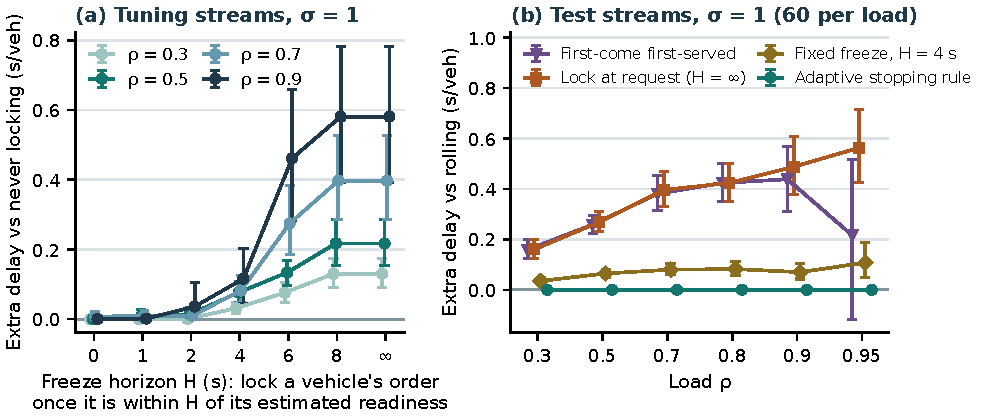
\includegraphics[width=\linewidth]{figures/fig2_commitment.pdf}
\caption{\textbf{Experiment A: the cost of locking crossing orders} (instantaneous installation). (a) Tuning streams: extra mean delay of a freeze horizon against never locking. (b) Test streams: paired difference from rolling optimization. 95\% stream intervals.}\label{fig:commitment}
\end{figure}

\paragraph{Experiment B: atomic versus release-gated replacement.} Table~\ref{tab:sweep} isolates single decisions. On a perfect link, release-gated direct installation fell short of the atomic update at exactly the \nSweepShortDirect{} of \nSweepForks{} forks that reversed a pair, the decisions whose release graph has a cycle. Reorders were \nSweepReorderShare\% of improving forks; across the 12 regimes, direct installation lost \nSweepGapPerfectMin--\nSweepGapPerfectMax{} ms per vehicle per fork, at most \nSweepGapPerfectShareMax\% of the atomic saving. With 100 ms slots the loss grew steadily with the loss rate per leg, reaching \nSweepGapNineMin--\nSweepGapNineMax{} ms at 10\% (up to \nSweepGapNineShareMax\% of the atomic saving), as erased grants and acknowledgments left updates unfinished. An easier direct target never helped (at most \nSweepMenuMax{} ms over the nominal target): rolling schedules are packed, so no direct target can reorder a tight pair.

\begin{table}[t]\centering\small
\caption{\textbf{Experiments B and C at single decisions} ($\sigma=1$ s, $h_f=3$ s; 32 streams per load). Atomic saving and differences in ms per live vehicle per fork, 95\% intervals. Reorders: forks reversing a pair (in brackets: completable with one temporary booking). Detour: the temporary booking chosen for a perfect link.}\label{tab:sweep}
\resizebox{\linewidth}{!}{\begin{tabular}{@{}rrrr ll ll@{}}\toprule
& & & & \multicolumn{2}{c}{perfect link (no delay, no loss)} & \multicolumn{2}{c}{lossy link (100 ms, 10\% loss per leg)}\\\cmidrule(lr){5-6}\cmidrule(l){7-8}
$\rho$ & forks & reorders & atomic & lost by direct & gained by detour & lost by direct & gained by detour\\\midrule
0.5 & 1,340 & 36 (36) & 479 & 22.2 [9.6, 37.2] & 22.2 [9.6, 37.2] & 88.1 [66.0, 111.8] & $-$0.9 [$-$9.2, 8.2]\\
0.75 & 2,057 & 57 (53) & 233 & 19.8 [10.7, 30.4] & 19.0 [9.9, 29.7] & 54.7 [41.0, 69.2] & $-$5.8 [$-$14.1, 2.0]\\
0.9 & 2,471 & 46 (44) & 138 & 16.2 [8.2, 25.9] & 15.7 [7.6, 25.4] & 36.0 [23.3, 50.1] & $-$3.3 [$-$10.7, 3.6]\\
\bottomrule\end{tabular}
}
\end{table}

\paragraph{Experiment C: temporary reservations.} On a perfect link, one temporary booking completed \nSweepRescued{} of the \nSweepReorders{} cyclic forks (\nSweepRescuedShare\%) and recovered \nSweepRecMin--\nSweepRecMax{} ms per vehicle per fork across regimes, nearly all of the structural loss. With one attempt per message the same detours became a liability (Fig.~\ref{fig:detours}). In the example of Fig.~\ref{fig:handoff} at $u=v=0.9$, Eq.~\eqref{eq:value} values the detour at \nPairNine{} vehicle-seconds against 0.9 for the best direct target, and it stops paying at \nPairCross\% loss per leg: a detour is a chain of three dependent messages, and its park move, which delays a vehicle, succeeds more often than its return. At 10\% loss, detours chosen for a perfect link had a negative effect in all 12 regimes, with the interval below zero in \nSweepObliviousNeg{} of them. Scoring detours by Eq.~\eqref{eq:value} avoided these losses (its estimated effect against direct installation was non-negative in \nSweepAwareNonNeg{} of 12 regimes), but the gain of the loss-aware choice over the best direct target was not significant (\nSweepPrimary{} ms [\nSweepPrimaryLo, \nSweepPrimaryHi] at the base cell; no regime survived Holm correction). In sustained traffic (Table~\ref{tab:recovery}) temporary bookings with one attempt added \nRtDetourZeroLowAbs{} and \nRtDetourZeroHighAbs{} s per vehicle ($\rho=0.5$, $0.75$), but with two retries they reduced delay by \nRtDetourTwoLowAbs{} and \nRtDetourTwoHighAbs{} s ($\rho=0.75$: [\nRtDetourTwoHighLo, \nRtDetourTwoHighHi]), the best safe method we tested: retries rescue chains.

\begin{figure}[t]\centering
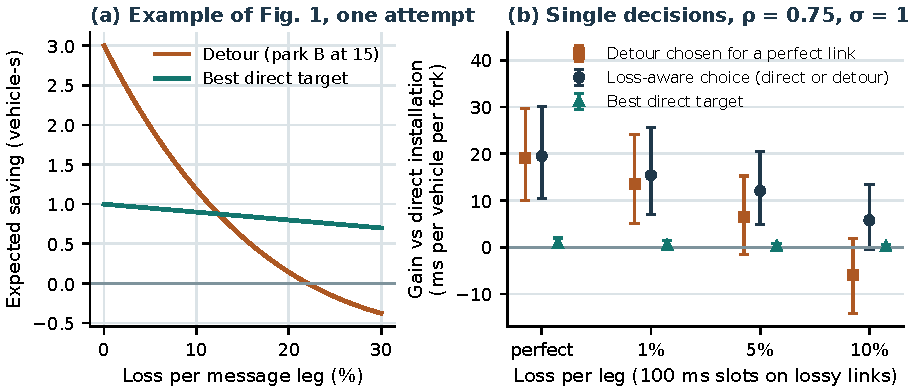
\includegraphics[width=\linewidth]{figures/fig3_detours.pdf}
\caption{\textbf{Experiment C: when does a temporary reservation pay?} (a) Expected saving in the example of Fig.~\ref{fig:handoff} with one attempt per message, from Eq.~\eqref{eq:value}. (b) Forks at $\rho=0.75$, $\sigma=1$ s (\nSweepPrimaryForks{} forks): gain over direct installation of the nominal target by link quality. 95\% stream intervals.}\label{fig:detours}
\end{figure}

\paragraph{Experiment D: communication loss and recovery.} Fig.~\ref{fig:recovery}a and Table~\ref{tab:recovery} report the price of safe installation, the extra mean delay against the idealized instantaneous update. On a clean 100 ms link the one-attempt protocol cost \nRtPriceZeroCleanLow{} and \nRtPriceZeroCleanHigh{} s per vehicle at $\rho=0.5$ and $0.75$, the structural and latency cost of serialized single moves. At 10\% loss it cost \nRtPriceZeroTenLow{} and \nRtPriceZeroTenHigh{} s, worse than instantaneous FCFS, because \nRtPinnedZero{} vehicles per stream ($\rho=0.75$) were left pinned with two protected bookings. The main comparison, one retry minus one attempt at $\rho=0.75$, $d=0.1$ s and 10\% loss, was \nRtPrimary{} s per vehicle [\nRtPrimaryLo, \nRtPrimaryHi] ($p<\nRtPrimaryP$), \nRtRecOne\% [\nRtRecOneLo, \nRtRecOneHi] of the one-attempt price. Two retries recovered \nRtRecTwo\% and left \nRtPriceTwoTenHigh{} s, only \nRtTwoTenMinusCleanHighAbs{} s [\nRtTwoTenMinusCleanHighLo, \nRtTwoTenMinusCleanHighHi] above the clean link. The oracle, which removes ambiguity entirely, recovered \nRtRecOracle\%, so nearly all of the loss-attributable price was ambiguity. Pinned vehicles fell from \nRtPinnedZero{} to \nRtPinnedOne{} and \nRtPinnedTwo{} per stream, in line with a round failing to confirm with probability $1-uv=0.19$. Recovery cost \nRtRetxOne{} and \nRtRetxTwo{} retransmissions per stream (\nRtRetxShareOne\% and \nRtRetxShareTwo\% of grants), and the 95th-percentile delay fell from \nRtPFiveZero{} to \nRtPFiveTwo{} s. At 20\% loss two retries left \nRtPriceTwoTwentyHigh{} s against \nRtPriceOracleTwentyHigh{} s for the oracle; with correlated loss (a lost leg is lost again with probability 0.5) one retry gained \nRtBurstOneAbs{} s instead of \nRtPrimaryAbs{} s. The time-aware rule never differed from two blind retries by more than \nRtAwareMax{} s per vehicle, because direct revisions advance vehicles and almost never contain the sacrifices it would withhold.

\begin{figure}[t]\centering
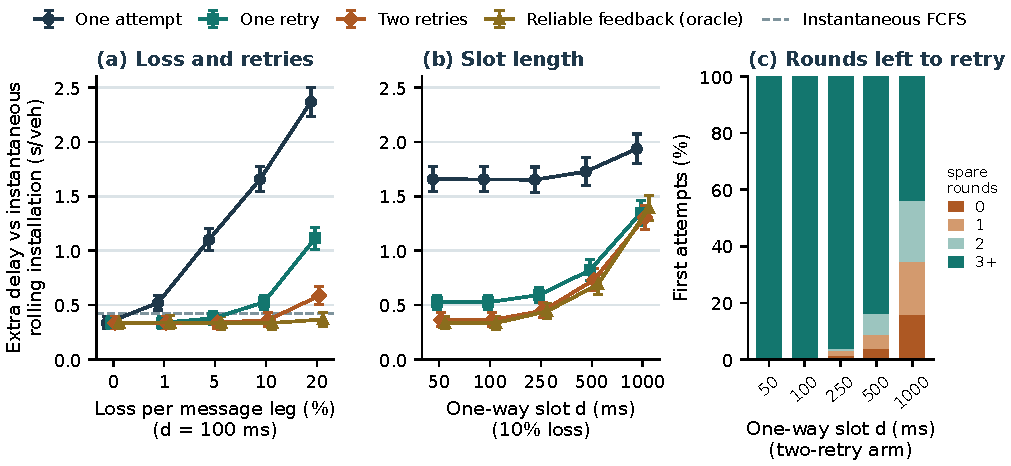
\includegraphics[width=\linewidth]{figures/fig4_recovery_deadlines.pdf}
\caption{\textbf{Experiments D and E} ($\rho=0.75$; 60 streams per cell; 95\% paired intervals). Extra mean delay against instantaneous rolling installation (a) by loss per message leg and (b) by one-way slot length. (c) First attempts by the number of further rounds in which a retry would still be physically certified (descriptive strata).}\label{fig:recovery}
\end{figure}

\begin{table}[t]\centering\small
\caption{\textbf{Sustained traffic at 10\% loss per leg, 100 ms slots} (60 streams per cell). Mean cohort delay and extra delay against instantaneous rolling (s per vehicle); pinned vehicles and retransmissions plus queries (retx) per stream.}\label{tab:recovery}
\begin{tabular}{@{}lrrrrrrrr@{}}\toprule
& \multicolumn{4}{c}{$\rho=0.5$} & \multicolumn{4}{c}{$\rho=0.75$}\\\cmidrule(lr){2-5}\cmidrule(l){6-9}
Installation & delay & extra & pinned & retx & delay & extra & pinned & retx\\\midrule
Instantaneous rolling (idealized) & 1.77 & -- & -- & -- & 4.92 & -- & -- & --\\
Instantaneous FCFS (idealized) & 2.06 & +0.29 & -- & -- & 5.34 & +0.43 & -- & --\\
\addlinespace
Safe installation, one attempt & 3.04 & +1.27 & 40.9 & 0 & 6.57 & +1.66 & 38.6 & 0\\
\quad with one retry & 2.16 & +0.39 & 9.7 & 51 & 5.44 & +0.53 & 9.2 & 50\\
\quad with two retries & 2.00 & +0.23 & 1.9 & 62 & 5.28 & +0.36 & 1.6 & 62\\
\quad with reliable feedback (oracle) & 2.00 & +0.23 & 0.0 & 0 & 5.25 & +0.34 & 0.0 & 0\\
\addlinespace
Temporary bookings, one attempt & 3.11 & +1.34 & 42.6 & 0 & 6.67 & +1.75 & 40.2 & 0\\
Temporary bookings, two retries & 1.90 & +0.13 & 2.0 & 67 & 5.14 & +0.22 & 1.9 & 67\\
Lock every order, one attempt & 3.10 & +1.33 & 40.4 & 0 & 6.64 & +1.72 & 38.0 & 0\\
Lock every order, one retry & 2.25 & +0.48 & 9.6 & 50 & 5.53 & +0.61 & 9.1 & 50\\
\bottomrule\end{tabular}

\end{table}

\paragraph{Experiment E: physical deadlines.} A retry needs a later switch instant at which the vehicle can still execute the change. With 100 ms slots, \nRtSpareThreeTenth\% of first attempts had three or more further certifiable rounds, and among their failures one and two retries resolved \nRtRecAmpleOne\% and \nRtRecAmpleTwo\%, close to the model's \nRtModelRecOne\% and \nRtModelRecTwo\%. That share fell to \nRtSpareThreeHalf\% at 0.5 s slots and \nRtSpareThreeSecond\% at 1 s, where \nRtSpareZeroSecond\% of first attempts had no usable retry at all (Fig.~\ref{fig:recovery}c). The benefit of one retry shrank from \nRtSlotFiftyOneHighAbs{} s per vehicle at 50 ms to \nRtSlotSecondOneHighAbs{} s at 1 s, where two retries still left \nRtSlotSecondPriceTwoHigh{} s against \nRtSlotSecondPriceZeroHigh{} s with one attempt (Fig.~\ref{fig:recovery}b). Longer rounds also slow every transaction, so the oracle degrades as well: deadlines are a real limit, but only for slots far longer than typical vehicle-to-infrastructure latencies.

\paragraph{Commitment under recovery, and limitations.} Locking every order did not become useful when revision was costly: it added \nRtFreezeZeroLowAbs{} and \nRtFreezeZeroHighAbs{} s per vehicle with one attempt and \nRtFreezeOneLowAbs{} and \nRtFreezeOneHighAbs{} s with one retry ($\rho=0.75$: [\nRtFreezeOneHighLo, \nRtFreezeOneHighHi]). Fork-level results (B, C) and sustained-traffic results (D, E) measure different quantities (saving at one decision versus mean delay of a cohort) and are never combined. All results come from a simulator with one conflict zone, synthetic erasures, bounded delay, synchronized clocks, exact tracking, cooperative vehicles and reliable first bookings.

\section{Contribution}\label{sec:contrib}
Table~\ref{tab:contrib} lists the tasks assigned to each team member and whether they were fulfilled. Every member completed all of their assigned tasks.

\begin{table}[h]\centering\small
\caption{Tasks assigned to each team member and their fulfilment.}\label{tab:contrib}
\begin{tabularx}{\linewidth}{@{}l>{\raggedright\arraybackslash}Xc@{}}\toprule
Member & Assigned tasks & Fulfilled \\\midrule
Nishchay Bhutoria (23110222) & Research idea and conceptualization; mathematical formulation; scheduling and coordination algorithm design; safe reservation revision and execution-aware decisions; methodology and experimental design; integration and interpretation of findings; technical direction & Yes \\
Tanish Wanve (23110327) & Vehicle and intersection simulation; vehicle-dynamics constraints and scheduling environment; baseline algorithms and tests; simulation validation and correctness checks; simulator integration & Yes \\
Swayam Borate (23110066) & Experiment configuration and execution; benchmark comparisons; statistical analysis; results processing and visualization; reproducibility checks & Yes \\
D A S K R Manognya (24110097) & Literature review and comparison; testing and validation documentation; report organization, references and presentation; repository documentation and reproduction instructions; preparation of results & Yes \\\bottomrule
\end{tabularx}\end{table}

\section{Conclusion}
A better crossing schedule is an opportunity, not an authorization. When every change must be installed safely, message by message, the benefit of re-optimization depends on the structure of the change and on whether the protocol can learn what actually happened. In our model, flexible orders always beat locked ones; order-preserving revisions installed almost for free, while reversals of tight pairs needed a temporary reservation; and under message loss, ambiguity rather than optimization dominated the price of safe revision. Bounded, version-safe retries removed most of that price, made temporary reservations worthwhile, and were limited by physical deadlines only for long message slots. The main limitation is the model: one conflict zone with idealized clocks and tracking and synthetic erasures; multiple conflict points and measured channels are the natural next steps. The code, data and instructions for reproducing every result are available at \url{https://github.com/nishchaybhutoria/FAI_Final}.

\bibliographystyle{unsrtnat}
\bibliography{references}
\end{document}
